% This is the Reed College LaTeX thesis template. Most of the work
% for the document class was done by Sam Noble (SN), as well as this
% template. Later comments etc. by Ben Salzberg (BTS). Additional
% restructuring and APA support by Jess Youngberg (JY).
% Your comments and suggestions are more than welcome; please email
% them to cus@reed.edu
%
% See http://web.reed.edu/cis/help/latex.html for help. There are a
% great bunch of help pages there, with notes on
% getting started, bibtex, etc. Go there and read it if you're not
% already familiar with LaTeX.
%
% Any line that starts with a percent symbol is a comment.
% They won't show up in the document, and are useful for notes
% to yourself and explaining commands.
% Commenting also removes a line from the document;
% very handy for troubleshooting problems. -BTS

% As far as I know, this follows the requirements laid out in
% the 2002-2003 Senior Handbook. Ask a librarian to check the
% document before binding. -SN

%%
%% Preamble
%%
% \documentclass{<something>} must begin each LaTeX document
\documentclass[12pt,twoside]{reedthesis}
% Packages are extensions to the basic LaTeX functions. Whatever you
% want to typeset, there is probably a package out there for it.
% Chemistry (chemtex), screenplays, you name it.
% Check out CTAN to see: http://www.ctan.org/
%%
\usepackage{graphicx,latexsym}
\usepackage[french]{babel} 
\usepackage{amsmath}
\usepackage{amssymb,amsthm}
\usepackage{xcolor}
\usepackage{eso-pic}
\usepackage{longtable,booktabs,setspace}
\usepackage{chemarr} %% Useful for one reaction arrow, useless if you're not a chem major
\usepackage[hyphens]{url}
\usepackage{tikz}
\usetikzlibrary{calc}
\newcommand\HRule{\rule{\textwidth}{1pt}}
% Added by CII
\usepackage{hyperref}
\usepackage{lmodern}
\usepackage{float}
\floatplacement{figure}{H}
% End of CII addition
\usepackage{rotating}

% Next line commented out by CII
%%% \usepackage{natbib}
% Comment out the natbib line above and uncomment the following two lines to use the new
% biblatex-chicago style, for Chicago A. Also make some changes at the end where the
% bibliography is included.
%\usepackage{biblatex-chicago}
%\bibliography{thesis}


% Added by CII (Thanks, Hadley!)
% Use ref for internal links
\renewcommand{\hyperref}[2][???]{\autoref{#1}}
\def\chapterautorefname{Chapter}
\def\sectionautorefname{Section}
\def\subsectionautorefname{Subsection}
% End of CII addition

% Added by CII
\usepackage{caption}
\captionsetup{width=5in}
% End of CII addition

% \usepackage{times} % other fonts are available like times, bookman, charter, palatino


% To pass between YAML and LaTeX the dollar signs are added by CII
\title{THÈSE}
\author{Thomas Karaouzene}
\labo{}
% The month and year that you submit your FINAL draft TO THE LIBRARY (May or December)
\date{31 octobre 2017}
\division{}
\advisor{Pierre Ray}
%If you have two advisors for some reason, you can use the following
% Uncommented out by CII
\altadvisor{Nicolas Thierry-Mieg}
% End of CII addition

%%% Remember to use the correct department!
\department{Ingénierie de la Santé, de la Cognition et Environnement (EDISCE)}
% if you're writing a thesis in an interdisciplinary major,
% uncomment the line below and change the text as appropriate.
% check the Senior Handbook if unsure.
%\thedivisionof{The Established Interdisciplinary Committee for}
% if you want the approval page to say "Approved for the Committee",
% uncomment the next line
%\approvedforthe{Committee}

% Added by CII
%%% Copied from knitr
%% maxwidth is the original width if it's less than linewidth
%% otherwise use linewidth (to make sure the graphics do not exceed the margin)
\makeatletter
\def\maxwidth{ %
  \ifdim\Gin@nat@width>\linewidth
    \linewidth
  \else
    \Gin@nat@width
  \fi
}
\makeatother

\renewcommand{\contentsname}{Table of Contents}
% End of CII addition

\setlength{\parskip}{0pt}

% Added by CII

\providecommand{\tightlist}{%
  \setlength{\itemsep}{0pt}\setlength{\parskip}{0pt}}

\Acknowledgements{

}

\Dedication{

}

\Preface{
This is an example of a thesis setup to use the reed thesis document
class (for LaTeX) and the R bookdown package, in general.
}

\Abstract{

}

% End of CII addition
%%
%% End Preamble
%%
%

\usepackage{amsthm}
\newtheorem{theorem}{Theorem}[section]
\newtheorem{lemma}{Lemma}[section]
\theoremstyle{definition}
\newtheorem{definition}{Definition}[section]
\newtheorem{corollary}{Corollary}[section]
\newtheorem{proposition}{Proposition}[section]
\theoremstyle{definition}
\newtheorem{example}{Example}[section]
\theoremstyle{remark}
\newtheorem*{remark}{Remark}
\begin{document}

% Everything below added by CII
      \maketitle
  
  \frontmatter % this stuff will be roman-numbered
  \pagestyle{empty} % this removes page numbers from the frontmatter

  
      \begin{preface}
      This is an example of a thesis setup to use the reed thesis document
      class (for LaTeX) and the R bookdown package, in general.
    \end{preface}
  
      \hypersetup{linkcolor=black}
    \setcounter{tocdepth}{2}
    \tableofcontents
  
      \listoftables
  
      \listoffigures
  
  
  
  \mainmatter % here the regular arabic numbering starts
  \pagestyle{fancyplain} % turns page numbering back on

  --\textgreater{}
  
  \chapter*{Remerciements}\label{remerciements}
  \addcontentsline{toc}{chapter}{Remerciements}
  
  Je remercie \ldots{}
  
  \newpage  
  
  ~
  
  ~
  
  ~
  
  ~
  
  ~
  
  ~
  
  ~
  
  ~
  
  ~
  
  ~
  
  ~
  
  ~
  
  ~
  
  ~
  
  ~
  
  ~
  
  ~
  
  ~
  
  ~
  
  ~
  
  ~
  
  ~
  
  ~
  
  ~
  
  ~
  
  ~
  
  ~
  
  ~
  
  ~
  
  ~
  
  ~
  
  ~
  
  ~
  
  ~
  
  ~
  
  ~
  
  ~
  
  ~
  
  ~
  
  ~
  
  ~
  
  ~
  
  ~
  
  \begin{verbatim}
                        Cette thèse est dédiée à ...
  \end{verbatim}
  
  \chapter*{Résumé}\label{resume}
  \addcontentsline{toc}{chapter}{Résumé}
  
  The preface pretty much says it all. \par
  
  Second paragraph of abstract starts here.
  
  \chapter*{Abstract}\label{abstract}
  \addcontentsline{toc}{chapter}{Abstract}
  
  The preface pretty much says it all. \par
  
  Second paragraph of abstract starts here.
  
  \chapter{Introduction}\label{introInf}
  
  \section{Structure et fonction du
  spermatozoïde}\label{structure-et-fonction-du-spermatozoide}
  
  \subsection{La spermatogénèse}\label{la-spermatogenese}
  
  La spermatogenèse des mamifères est un processus long et complexe
  controllé par plusieurs mécanismes étroitement liés ((Gnessi, Fabbri, \&
  Spera, 1997, Kierszenbaum (1994)),\textbf{Sharpe1994 à trouver!!!}).
  C'est au cours de celle-ci que, à partir de cellules germinales, seront
  produits les spermatozoïdes matures. Ce processus est divisé en trois
  phases principales : La phase de multiplication, la phase de division
  (appelée la méiose) et la phase de maturation. Chez les hommes, ces
  tapes se déroulent en continue dans la paroi des tubes séminifères du
  testicules depuis la pubertés jusqu'à la mort et implique trois types de
  cellules germinales : les spermatogonies, les spermatocytes et les
  spermatides. Le temps nécessaire pour obtenir un spermatozoïde mature à
  partir de cellules germinales est de 74 jours et la production
  quotidienne de spermatozoïde est d'environ 45 million par testicules
  (Johnson, Petty, \& Neaves, 1980).
  
  \subsubsection{Rappels sur le testicule}\label{rappels-sur-le-testicule}
  
  Les testicules sont les organes sexuels masculins. Ils possèdes deux
  fonctions principales plus ou moins exprimés selon les période de la vie
  de l'individu : une fonction endocrine caractérisé par la synthèse des
  hormones stéroïdes sexuelles masculines (la stéroïdogenèse) et une
  fonction exocrine au cours de laquelle seront produits les gamètes
  masculins. Chez un individu adulte en bonne santé, celui-ci présente une
  forme ovoïde ayant un volume moyen de 18
  cm\textsuperscript{\textsuperscript{3}} par testicule. Comme chez la
  plupart des mammifères terrestres, ils sont sous le pénis dans dans une
  poche de peau appelée scrotum et reliés à l'abdomen par le cordon
  spermatique (Figure : \ref{fig:testicule}). Cette externalisation des
  testicules permet leur maintien à une température plus basse que celle
  du reste du corps nécessaire à la spermatogenèse.\\
  L'intérieur du testicule contient des tubes séminifères enroulés ainsi
  que du tissu entre les tubules appelé espace interstitiel. Les tubes
  séminifères sont de longs tubes compactés sous forme de boucles et dont
  les deux extrémités débouchent sur le \emph{rete testis} (Figure :
  \ref{fig:testicule}). C'est le long des parois du tube séminifère que se
  dérouleront l'ensemble des étapes de la spermatogenèse.
  
  \begin{figure}
  
  {\centering 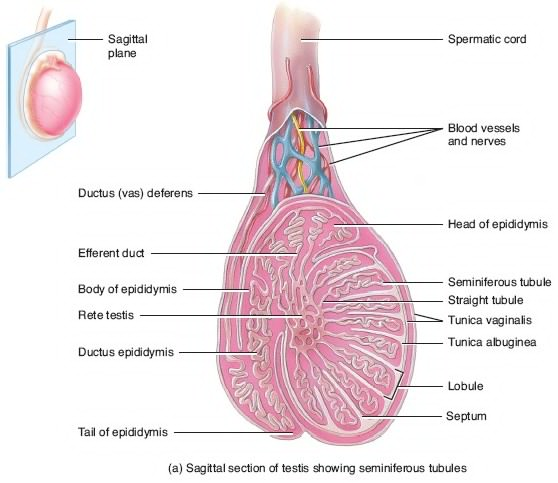
\includegraphics[scale=0.65]{figure/coupe_testicule2} 
  
  }
  
  \caption{Schéma anatomique du testicule humain : }\label{fig:testicule}
  \end{figure}
  
  \subsubsection{La phase de
  multiplication}\label{la-phase-de-multiplication}
  
  La phase de multiplication est la phase au cours de laquelle les
  spermatogonies se divisent par mitoses pour aboutir au stade de
  spermatocytes primaires. Les spermatogonies sont des cellules dploïdes à
  l'origine de k'ensemble des autres cellules germinales humaines. Pour
  cela, elle vont s'auto-renouveller par mitose successive afin de
  maintenir une production continue de spermatozoïdes tout au long de la
  vie de l'individu. Ces cellules sont localisées dans le compartiment
  basal des tubes séminifères. Elles présentent un noyau ovoïde ainsi
  qu'un cytoplasme dense contenant un petit appareil de Golgi, quelques
  mitochondrie ainsqi que plusieurs ribosomes libres. Les analyses
  histologiques ont permis de distinguer trois types de spermatogonies en
  fonction de leur contenu en heterochromatine ((Clermont, 1963, Clermont
  (1966), Goossens \& Tournaye (2013))) :
  
  \begin{enumerate}
  \def\labelenumi{\arabic{enumi}.}
  \tightlist
  \item
    Les spermatogonies de type A dark (ou Ad)\\
  \item
    Les spermatogonies de type A pale (ou Ap)\\
  \item
    Les spermatogonies de type B
  \end{enumerate}
  
  Dans le modèle le plus communément accepté, les spermatogonies Ad vont
  au cours d'une première mitose former un spermatogonie Ad et un
  spermatogonie Ap (\textbf{Figure :} \ref{fig:spermatogenese}). Cette
  propriété permet à la fois de se différencier en spermatocytes tout en
  constituant un compartiment de réserve de spermatogonies Ad permettant
  d'assurer la production permanente de spermatozoïdes. Les spermatogonies
  Ap ainsi formés se diviseront ensuite par mitose pour former deux
  spermatogonies B qui elles-mêmes se diviseront en deux spermatocytes
  primaires diploïdes (\textbf{Figure :} \ref{fig:spermatogenese}).
  
  \begin{figure}
  
  {\centering 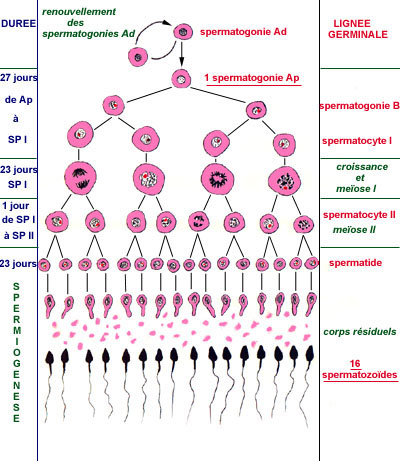
\includegraphics[scale=0.75]{figure/spermatogenese} 
  
  }
  
  \caption{Les différentes phases de la spermatogénèse}\label{fig:spermatogenese}
  \end{figure}
  
  \subsubsection{La méïose}\label{la-meiose}
  
  La méiose, ou phase de maturation, est l'étape au cours de laquelle, à
  partir de cellules diploïdes (les spermatogonies B) vont se former des
  cellules haploïdes, les spermatocytes secondaire (spermatocytes II).\\
  Ce résultat est le fruit de deux divisions succesives (\textbf{Figure :
  }\ref{fig:meiose}) appellée respectivement méïose réductionnelle ou
  méiose I (MI) et méiose équationnelle ou méiose II (MII). La MI va
  séparer les chromosomes homologues, produisant deux cellules haploïdes.
  
  \begin{figure}
  
  {\centering 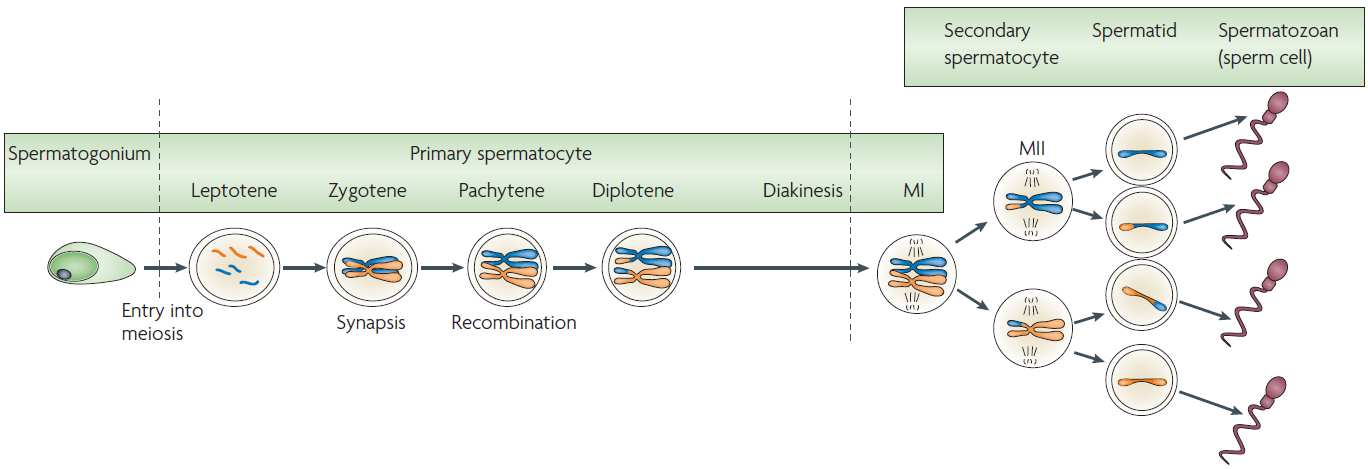
\includegraphics[scale=0.35]{figure/Meiosis_Stages} 
  
  }
  
  \caption{Les différentes étapes de la méiose gamétique masculine. D’après Sasaki et Matsui,
  2008}\label{fig:meiose}
  \end{figure}
  
  \subsubsection{La spermiogénèse}\label{la-spermiogenese}
  
  \subsection{Anatomie du spermatozoïde}\label{anatomie-du-spermatozoide}
  
  \begin{figure}
  
  {\centering 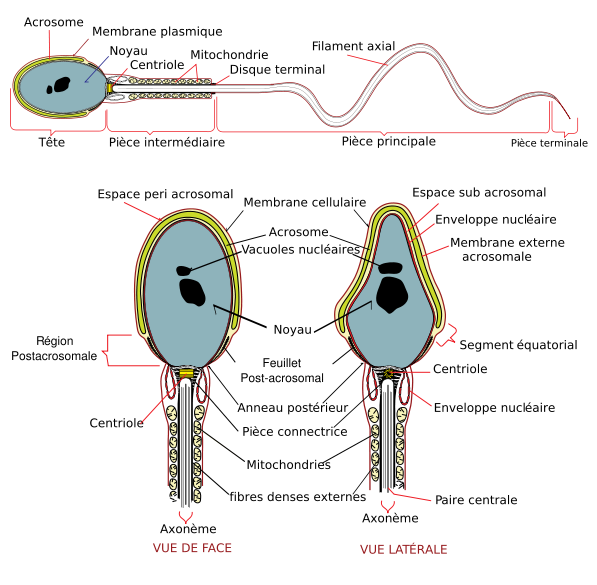
\includegraphics[scale=0.7]{figure/spermatozoide} 
  
  }
  
  \caption{Anatomie du spermatozoïde}\label{fig:spermatozoïde}
  \end{figure}
  
  \subsubsection{La tête}\label{la-tete}
  
  \subsubsection{Le flagelle}\label{le-flagelle}
  
  \subsection{Fonction du spermatozoïde}\label{fonction-du-spermatozoide}
  
  \section{L'infertilité masculine}\label{linfertilite-masculine}
  
  L'organisation mondiale de la santé définie l'infertilité comme étant :
  ``\emph{une pathologie du système reproductif définie par l'échec d'une
  grossesse clinique après 12 mois ou plus de rapports sexuels réguliers
  non protégés}''
  (\href{http://www.who.int/reproductivehealth/topics/infertility/definitions/en/}{\texttt{Who.int.\ 2013-03-19.\ Retrieved\ 2013-06-17}}).
  Environ 10-15\% des couples humains sont considérés infertiles. On
  estime que dans la moitié des cas, la cause sous-jacente est masculine.
  Les facteurs causaux sous-jacents de l'infertilité masculine peuvent
  être attribués à des toxines environnementales, des troubles systémiques
  tels que la maladie hypothalamo-hypophysaire, les cancers testiculaires
  et l'aplasie des cellules germinales. Les facteurs génétiques, y compris
  les aneuploïdies et les mutations de gènes uniques, contribuent
  également à l'infertilité masculine. Cependant, aucune cause n'est
  identifiée dans 10-20\% des cas.
  
  \subsection{Les différents phénotypes d'infertilité
  masculine}\label{les-differents-phenotypes-dinfertilite-masculine}
  
  \subsubsection{Liée à la quantité}\label{liee-a-la-quantite}
  
  \subsubsection{liée à la forme}\label{liee-a-la-forme}
  
  \subsubsection{liée à la mobilitée}\label{liee-a-la-mobilitee}
  
  \subsection{La génétique de
  l'infertilité}\label{la-genetique-de-linfertilite}
  
  \subsubsection{Les causes fréquentes}\label{les-causes-frequentes}
  
  \paragraph{Les microdélétions du chromosome
  Y}\label{les-microdeletions-du-chromosome-y}
  
  \paragraph{Anomalies chromosomiques}\label{anomalies-chromosomiques}
  
  \paragraph{Mutations CFTR}\label{mutations-cftr}
  
  \subsubsection{Les nouveaux gènes}\label{les-nouveaux-genes}
  
  \begin{center}\rule{0.5\linewidth}{\linethickness}\end{center}
  
  \section{Les techniques d'analyses
  génétiques}\label{les-techniques-danalyses-genetiques}
  
  \subsection{Les puces}\label{les-puces}
  
  \subsection{Le séquençage}\label{le-sequencage}
  
  \subsubsection{Le Sanger}\label{le-sanger}
  
  \subsubsection{Le NGS}\label{le-ngs}
  
  \begin{center}\rule{0.5\linewidth}{\linethickness}\end{center}
  
  \section{L'analyse bioinformatique}\label{lanalyse-bioinformatique}
  
  \subsection{L'analyse des données brut}\label{lanalyse-des-donnees-brut}
  
  \subsubsection{L'alignement}\label{lalignement}
  
  \subsubsection{L'appel des variants}\label{lappel-des-variants}
  
  \subsection{La priorisation des
  variants}\label{la-priorisation-des-variants}
  
  \chapter{Investigation génétique et physiologique de la
  globozoospermie}\label{globo}
  
  \section{Math}\label{math}
  
  \section{Chemistry 101: Symbols}\label{chemistry-101-symbols}
  
  Chemical formulas will look best if they are not italicized. Get around
  math mode's automatic italicizing in LaTeX by using the argument
  \texttt{\$\textbackslash{}mathrm\{formula\ here\}\$}, with your formula
  inside the curly brackets. (Notice the use of the backticks here which
  enclose text that acts as code.)
  
  So, \(\mathrm{Fe_2^{2+}Cr_2O_4}\) is written
  \texttt{\$\textbackslash{}mathrm\{Fe\_2\^{}\{2+\}Cr\_2O\_4\}\$}.
  
  \noindent Exponent or Superscript: \(\mathrm{O^-}\)
  
  \noindent Subscript: \(\mathrm{CH_4}\)
  
  To stack numbers or letters as in \(\mathrm{Fe_2^{2+}}\), the subscript
  is defined first, and then the superscript is defined.
  
  \noindent Bullet: CuCl \(\bullet\) \(\mathrm{7H_{2}O}\)
  
  \noindent Delta: \(\Delta\)
  
  \noindent Reaction Arrows: \(\longrightarrow\) or
  \(\xrightarrow{solution}\)
  
  \noindent Resonance Arrows: \(\leftrightarrow\)
  
  \noindent Reversible Reaction Arrows: \(\rightleftharpoons\)
  
  \subsection{Typesetting reactions}\label{typesetting-reactions}
  
  You may wish to put your reaction in an equation environment, which
  means that LaTeX will place the reaction where it fits and will number
  the equations for you.
  
  \begin{equation}
    \mathrm{C_6H_{12}O_6  + 6O_2} \longrightarrow \mathrm{6CO_2 + 6H_2O}
    \label{eq:reaction}
  \end{equation}
  
  We can reference this combustion of glucose reaction via Equation
  \eqref{eq:reaction}.
  
  \subsection{Other examples of
  reactions}\label{other-examples-of-reactions}
  
  \(\mathrm{NH_4Cl_{(s)}}\) \(\rightleftharpoons\)
  \(\mathrm{NH_{3(g)}+HCl_{(g)}}\)
  
  \noindent \(\mathrm{MeCH_2Br + Mg}\) \(\xrightarrow[below]{above}\)
  \(\mathrm{MeCH_2\bullet Mg \bullet Br}\)
  
  \section{Physics}\label{physics}
  
  Many of the symbols you will need can be found on the math page
  \url{http://web.reed.edu/cis/help/latex/math.html} and the Comprehensive
  LaTeX Symbol Guide
  (\url{http://mirror.utexas.edu/ctan/info/symbols/comprehensive/symbols-letter.pdf}).
  
  \section{Biology}\label{biology}
  
  You will probably find the resources at
  \url{http://www.lecb.ncifcrf.gov/~toms/latex.html} helpful, particularly
  the links to bsts for various journals. You may also be interested in
  TeXShade for nucleotide typesetting
  (\url{http://homepages.uni-tuebingen.de/beitz/txe.html}). Be sure to
  read the proceeding chapter on graphics and tables.
  
  \chapter{Tables, Graphics, References, and Labels}\label{ref-labels}
  
  \section{Tables}\label{tables}
  
  In addition to the tables that can be automatically generated from a
  data frame in \textbf{R} that you saw in {[}R Markdown Basics{]} using
  the \texttt{kable} function, you can also create tables using
  \emph{pandoc}. (More information is available at
  \url{http://pandoc.org/README.html\#tables}.) This might be useful if
  you don't have values specifically stored in \textbf{R}, but you'd like
  to display them in table form. Below is an example. Pay careful
  attention to the alignment in the table and hyphens to create the rows
  and columns.
  
  \begin{longtable}[]{@{}ccc@{}}
  \caption{\label{tab:inher} Correlation of Inheritance Factors for Parents
  and Child}\tabularnewline
  \toprule
  \begin{minipage}[b]{0.29\columnwidth}\centering\strut
  Factors\strut
  \end{minipage} & \begin{minipage}[b]{0.47\columnwidth}\centering\strut
  Correlation between Parents \& Child\strut
  \end{minipage} & \begin{minipage}[b]{0.16\columnwidth}\centering\strut
  Inherited\strut
  \end{minipage}\tabularnewline
  \midrule
  \endfirsthead
  \toprule
  \begin{minipage}[b]{0.29\columnwidth}\centering\strut
  Factors\strut
  \end{minipage} & \begin{minipage}[b]{0.47\columnwidth}\centering\strut
  Correlation between Parents \& Child\strut
  \end{minipage} & \begin{minipage}[b]{0.16\columnwidth}\centering\strut
  Inherited\strut
  \end{minipage}\tabularnewline
  \midrule
  \endhead
  \begin{minipage}[t]{0.29\columnwidth}\centering\strut
  Education\strut
  \end{minipage} & \begin{minipage}[t]{0.47\columnwidth}\centering\strut
  -0.49\strut
  \end{minipage} & \begin{minipage}[t]{0.16\columnwidth}\centering\strut
  Yes\strut
  \end{minipage}\tabularnewline
  \begin{minipage}[t]{0.29\columnwidth}\centering\strut
  Socio-Economic Status\strut
  \end{minipage} & \begin{minipage}[t]{0.47\columnwidth}\centering\strut
  0.28\strut
  \end{minipage} & \begin{minipage}[t]{0.16\columnwidth}\centering\strut
  Slight\strut
  \end{minipage}\tabularnewline
  \begin{minipage}[t]{0.29\columnwidth}\centering\strut
  Income\strut
  \end{minipage} & \begin{minipage}[t]{0.47\columnwidth}\centering\strut
  0.08\strut
  \end{minipage} & \begin{minipage}[t]{0.16\columnwidth}\centering\strut
  No\strut
  \end{minipage}\tabularnewline
  \begin{minipage}[t]{0.29\columnwidth}\centering\strut
  Family Size\strut
  \end{minipage} & \begin{minipage}[t]{0.47\columnwidth}\centering\strut
  0.18\strut
  \end{minipage} & \begin{minipage}[t]{0.16\columnwidth}\centering\strut
  Slight\strut
  \end{minipage}\tabularnewline
  \begin{minipage}[t]{0.29\columnwidth}\centering\strut
  Occupational Prestige\strut
  \end{minipage} & \begin{minipage}[t]{0.47\columnwidth}\centering\strut
  0.21\strut
  \end{minipage} & \begin{minipage}[t]{0.16\columnwidth}\centering\strut
  Slight\strut
  \end{minipage}\tabularnewline
  \bottomrule
  \end{longtable}
  
  We can also create a link to the table by doing the following: Table
  \ref{tab:inher}. If you go back to {[}Loading and exploring data{]} and
  look at the \texttt{kable} table, we can create a reference to this max
  delays table too: Table \ref{tab:maxdelays}. The addition of the
  \texttt{(\textbackslash{}\#tab:inher)} option to the end of the table
  caption allows us to then make a reference to Table
  \texttt{\textbackslash{}@ref(tab:label)}. Note that this reference could
  appear anywhere throughout the document after the table has appeared.
  
  \clearpage
  
  \section{Figures}\label{figures}
  
  If your thesis has a lot of figures, \emph{R Markdown} might behave
  better for you than that other word processor. One perk is that it will
  automatically number the figures accordingly in each chapter. You'll
  also be able to create a label for each figure, add a caption, and then
  reference the figure in a way similar to what we saw with tables
  earlier. If you label your figures, you can move the figures around and
  \emph{R Markdown} will automatically adjust the numbering for you. No
  need for you to remember! So that you don't have to get too far into
  LaTeX to do this, a couple \textbf{R} functions have been created for
  you to assist. You'll see their use below.
  
  In the \textbf{R} chunk below, we will load in a picture stored as
  \texttt{reed.jpg} in our main directory. We then give it the caption of
  ``Reed logo'', the label of ``reedlogo'', and specify that this is a
  figure. Make note of the different \textbf{R} chunk options that are
  given in the R Markdown file (not shown in the knitted document).
  
  \begin{figure}[htbp]
  \centering
  \includegraphics{figure/reed.jpg}
  \caption{\label{fig:reedlogo}Reed logo}
  \end{figure}
  
  Here is a reference to the Reed logo: Figure \ref{fig:reedlogo}. Note
  the use of the \texttt{fig:} code here. By naming the \textbf{R} chunk
  that contains the figure, we can then reference that figure later as
  done in the first sentence here. We can also specify the caption for the
  figure via the R chunk option \texttt{fig.cap}.
  
  \clearpage 
  
  Below we will investigate how to save the output of an \textbf{R} plot
  and label it in a way similar to that done above. Recall the
  \texttt{flights} dataset from Chapter. (Note that we've shown a
  different way to reference a section or chapter here.) We will next
  explore a bar graph with the mean flight departure delays by airline
  from Portland for 2014. Note also the use of the \texttt{scale}
  parameter which is discussed on the next page.
  
  \begin{figure}[htbp]
  \centering
  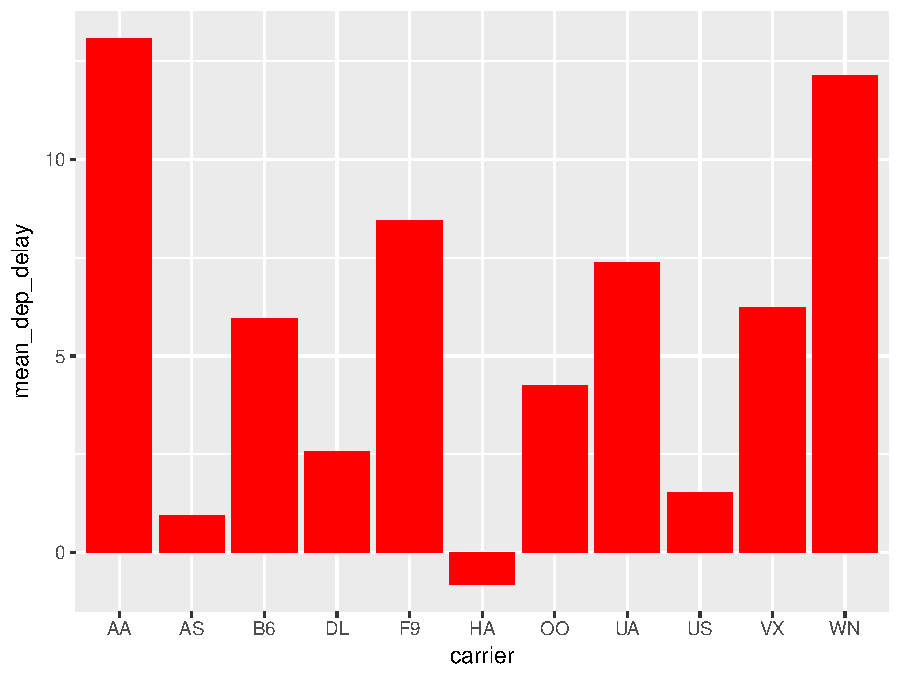
\includegraphics{thesis_files/figure-latex/delaysboxplot-1.pdf}
  \caption{\label{fig:delaysboxplot}Mean Delays by Airline}
  \end{figure}
  
  Here is a reference to this image: Figure \ref{fig:delaysboxplot}.
  
  A table linking these carrier codes to airline names is available at
  \url{https://github.com/ismayc/pnwflights14/blob/master/data/airlines.csv}.
  
  \clearpage
  
  Next, we will explore the use of the \texttt{out.extra} chunk option,
  which can be used to shrink or expand an image loaded from a file by
  specifying \texttt{"scale=\ "}. Here we use the mathematical graph
  stored in the ``subdivision.pdf'' file.
  
  \begin{figure}
  \includegraphics[scale=0.75]{figure/subdivision} \caption{Subdiv. graph}\label{fig:subd}
  \end{figure}
  
  Here is a reference to this image: Figure \ref{fig:subd}. Note that
  \texttt{echo=FALSE} is specified so that the \textbf{R} code is hidden
  in the document.
  
  \textbf{More Figure Stuff}
  
  Lastly, we will explore how to rotate and enlarge figures using the
  \texttt{out.extra} chunk option. (Currently this only works in the PDF
  version of the book.)
  
  \begin{figure}
  \includegraphics[angle=180, scale=1.1]{figure/subdivision} \caption{A Larger Figure, Flipped Upside Down}\label{fig:subd2}
  \end{figure}
  
  As another example, here is a reference: Figure \ref{fig:subd2}.
  
  \section{Footnotes and Endnotes}\label{footnotes-and-endnotes}
  
  You might want to footnote something.\footnote{footnote text} The
  footnote will be in a smaller font and placed appropriately. Endnotes
  work in much the same way. More information can be found about both on
  the CUS site or feel free to reach out to
  \href{mailto:data@reed.edu}{\nolinkurl{data@reed.edu}}.
  
  \section{Bibliographies}\label{bibliographies}
  
  Of course you will need to cite things, and you will probably accumulate
  an armful of sources. There are a variety of tools available for
  creating a bibliography database (stored with the .bib extension). In
  addition to BibTeX suggested below, you may want to consider using the
  free and easy-to-use tool called Zotero. The Reed librarians have
  created Zotero documentation at
  \url{http://libguides.reed.edu/citation/zotero}. In addition, a tutorial
  is available from Middlebury College at
  \url{http://sites.middlebury.edu/zoteromiddlebury/}.
  
  \emph{R Markdown} uses \emph{pandoc} (\url{http://pandoc.org/}) to build
  its bibliographies. One nice caveat of this is that you won't have to do
  a second compile to load in references as standard LaTeX requires. To
  cite references in your thesis (after creating your bibliography
  database), place the reference name inside square brackets and precede
  it by the ``at'' symbol. For example, here's a reference to a book about
  worrying: ({\textbf{???}}). This \texttt{Molina1994} entry appears in a
  file called \texttt{thesis.bib} in the \texttt{bib} folder. This
  bibliography database file was created by a program called BibTeX. You
  can call this file something else if you like (look at the YAML header
  in the main .Rmd file) and, by default, is to placed in the \texttt{bib}
  folder.
  
  For more information about BibTeX and bibliographies, see our CUS site
  (\url{http://web.reed.edu/cis/help/latex/index.html})\footnote{({\textbf{???}})}.
  There are three pages on this topic: \emph{bibtex} (which talks about
  using BibTeX, at \url{http://web.reed.edu/cis/help/latex/bibtex.html}),
  \emph{bibtexstyles} (about how to find and use the bibliography style
  that best suits your needs, at
  \url{http://web.reed.edu/cis/help/latex/bibtexstyles.html}) and
  \emph{bibman} (which covers how to make and maintain a bibliography by
  hand, without BibTeX, at
  \url{http://web.reed.edu/cis/help/latex/bibman.html}). The last page
  will not be useful unless you have only a few sources.
  
  If you look at the YAML header at the top of the main .Rmd file you can
  see that we can specify the style of the bibliography by referencing the
  appropriate csl file. You can download a variety of different style
  files at \url{https://www.zotero.org/styles}. Make sure to download the
  file into the csl folder.
  
  \textbf{Tips for Bibliographies}
  
  \begin{itemize}
  \tightlist
  \item
    Like with thesis formatting, the sooner you start compiling your
    bibliography for something as large as thesis, the better. Typing in
    source after source is mind-numbing enough; do you really want to do
    it for hours on end in late April? Think of it as procrastination.
  \item
    The cite key (a citation's label) needs to be unique from the other
    entries.
  \item
    When you have more than one author or editor, you need to separate
    each author's name by the word ``and'' e.g.
    \texttt{Author\ =\ \{Noble,\ Sam\ and\ Youngberg,\ Jessica\},}.
  \item
    Bibliographies made using BibTeX (whether manually or using a manager)
    accept LaTeX markup, so you can italicize and add symbols as
    necessary.
  \item
    To force capitalization in an article title or where all lowercase is
    generally used, bracket the capital letter in curly braces.
  \item
    You can add a Reed Thesis citation\footnote{({\textbf{???}})} option.
    The best way to do this is to use the phdthesis type of citation, and
    use the optional ``type'' field to enter ``Reed thesis'' or
    ``Undergraduate thesis.''
  \end{itemize}
  
  \section{Anything else?}\label{anything-else}
  
  If you'd like to see examples of other things in this template, please
  contact the Data @ Reed team (email
  \href{mailto:data@reed.edu}{\nolinkurl{data@reed.edu}}) with your
  suggestions. We love to see people using \emph{R Markdown} for their
  theses, and are happy to help.
  
  \chapter*{Conclusion}\label{conclusion}
  \addcontentsline{toc}{chapter}{Conclusion}
  
  If we don't want Conclusion to have a chapter number next to it, we can
  add the \texttt{\{-\}} attribute.
  
  \textbf{More info}
  
  And here's some other random info: the first paragraph after a chapter
  title or section head \emph{shouldn't be} indented, because indents are
  to tell the reader that you're starting a new paragraph. Since that's
  obvious after a chapter or section title, proper typesetting doesn't add
  an indent there.
  
  \appendix
  
  \chapter{The First Appendix}\label{the-first-appendix}
  
  This first appendix includes all of the R chunks of code that were
  hidden throughout the document (using the \texttt{include\ =\ FALSE}
  chunk tag) to help with readibility and/or setup.
  
  \textbf{In the main Rmd file}
  
  \textbf{In Chapter \ref{ref-labels}:}
  
  \begin{Shaded}
  \begin{Highlighting}[]
  \CommentTok{# This chunk ensures that the thesisdown package is}
  \CommentTok{# installed and loaded. This thesisdown package includes}
  \CommentTok{# the template files for the thesis and also two functions}
  \CommentTok{# used for labeling and referencing}
  \NormalTok{if(!}\KeywordTok{require}\NormalTok{(devtools))}
    \KeywordTok{install.packages}\NormalTok{(}\StringTok{"devtools"}\NormalTok{, }\DataTypeTok{repos =} \StringTok{"http://cran.rstudio.com"}\NormalTok{)}
  \NormalTok{if(!}\KeywordTok{require}\NormalTok{(dplyr))}
      \KeywordTok{install.packages}\NormalTok{(}\StringTok{"dplyr"}\NormalTok{, }\DataTypeTok{repos =} \StringTok{"http://cran.rstudio.com"}\NormalTok{)}
  \NormalTok{if(!}\KeywordTok{require}\NormalTok{(ggplot2))}
      \KeywordTok{install.packages}\NormalTok{(}\StringTok{"ggplot2"}\NormalTok{, }\DataTypeTok{repos =} \StringTok{"http://cran.rstudio.com"}\NormalTok{)}
  \NormalTok{if(!}\KeywordTok{require}\NormalTok{(ggplot2))}
      \KeywordTok{install.packages}\NormalTok{(}\StringTok{"bookdown"}\NormalTok{, }\DataTypeTok{repos =} \StringTok{"http://cran.rstudio.com"}\NormalTok{)}
  \NormalTok{if(!}\KeywordTok{require}\NormalTok{(thesisdown))\{}
    \KeywordTok{library}\NormalTok{(devtools)}
    \NormalTok{devtools::}\KeywordTok{install_github}\NormalTok{(}\StringTok{"ismayc/thesisdown"}\NormalTok{)}
    \NormalTok{\}}
  \KeywordTok{library}\NormalTok{(thesisdown)}
  \NormalTok{flights <-}\StringTok{ }\KeywordTok{read.csv}\NormalTok{(}\StringTok{"data/flights.csv"}\NormalTok{)}
  \end{Highlighting}
  \end{Shaded}
  
  \chapter{The Second Appendix, for
  Fun}\label{the-second-appendix-for-fun}
  
  \backmatter
  
  \chapter*{References}\label{references}
  \addcontentsline{toc}{chapter}{References}
  
  \noindent
  
  \setlength{\parindent}{-0.20in} \setlength{\leftskip}{0.20in}
  \setlength{\parskip}{8pt}
  
  \hypertarget{refs}{}
  \hypertarget{ref-Clermont1963}{}
  Clermont, Y. (1963). The cycle of the seminiferous epithelium in man.
  \emph{American Journal of Anatomy}, \emph{112}(1), 35--51.
  \url{http://doi.org/10.1002/aja.1001120103}
  
  \hypertarget{ref-Clermont1966}{}
  Clermont, Y. (1966). Renewal of spermatogonia in man. \emph{American
  Journal of Anatomy}, \emph{118}(2), 509--524.
  \url{http://doi.org/10.1002/aja.1001180211}
  
  \hypertarget{ref-Gnessi1997}{}
  Gnessi, L., Fabbri, A., \& Spera, G. (1997). Gonadal Peptides as
  Mediators of Development and Functional Control of the Testis: An
  Integrated System with Hormones and Local Environment
  \textless{}sup\textgreater{}1\textless{}/sup\textgreater{}.
  \emph{Endocrine Reviews}, \emph{18}(4), 541--609.
  \url{http://doi.org/10.1210/edrv.18.4.0310}
  
  \hypertarget{ref-Goossens2013}{}
  Goossens, E., \& Tournaye, H. (2013). Adult Stem Cells in the Human
  Testis. \emph{Seminars in Reproductive Medicine}, \emph{31}(01),
  039--048. \url{http://doi.org/10.1055/s-0032-1331796}
  
  \hypertarget{ref-Johnson1980}{}
  Johnson, L., Petty, C. S., \& Neaves, W. B. (1980). A comparative study
  of daily sperm production and testicular composition in humans and rats.
  \emph{Biology of Reproduction}, \emph{22}(5), 1233--43. Retrieved from
  \url{http://www.ncbi.nlm.nih.gov/pubmed/7417656}
  
  \hypertarget{ref-KIERSZENBAUM1994}{}
  Kierszenbaum, A. L. (1994). Mammalian Spermatogenesis in Vivo and in
  Vitro : A Partnership of Spermatogenic and Somatic Cell Lineages*.
  \emph{Endocrine Reviews}, \emph{15}(1), 116--134.
  \url{http://doi.org/10.1210/edrv-15-1-116}


  % Index?

\end{document}

